\section{Functional Description}
%----------------------- Functional description ----------------------------
\label{sec:functional_description}

This section provides an overview of the internal building blocks of Sesnando and how they inter


\subsection{Command Line Arguments}
%----------------------- Command Line Arguments ----------------------------
\label{subsec:command_line_arguments}

At the moment, Sesnando operates as a command line application. The command line arguments can be passed at the application launch, but a configuration file can be set, so that the user can define a set of default parameters avoiding the need to pass the arguments at all times. Default values from the configuration file will be used when omitting these parameters from the command line. The available command line arguments are defined on Table \ref{tab:CLI}.

As \textit{Sesnando} can be executed following a set of parameters from the command line or from a \textit{JSON} configuration, a detailed description of these commands are as follows.

\begin{itemize}
    \item signal\_manager - The address of the remote Signal Manager server, containing the data required to successfully generate test cases. Default port 5001.
    \item input - The location of the input file containing the requirements to be parsed by \textit{Sesnando}.
    \item output\_folder - The default location for the artifacts generated by \textit{Sesnando} (Can be overriden using "Save as..." from the test designer).
    \item test\_designer - The location of the Test Designer GUI module (usually on the same folder as the compiler binaries).
    \item debug - Debug mode mode allows a verbose execution of \textit{Sesnando}.
    \item neg\_testing - Negative testing True/False. Not all requirements require a negative testing verification. This will be discussed on Sec. \ref{sec:method}.
\end{itemize}

\begin{table}[H]
\caption{Sesnando Config parameters}
    \footnotesize
    \centering
    
    \begin{tabular}{c c c}
        \hline
        % --- ROW 1 --- %
        \textbf{\textit{Command}} & 
        \textbf{\textit{Default Value}} & 
        \textbf{\textit{Description}}\\ \hline  \\
        
        % --- ROW 2 --- %
        \begin{tabular}[c]{@{}c@{}} \textbf{\textit{-sm }} \textbf{\textit{--signal\_manager}}\end{tabular} & 
        127.0.0.1 & 
        Signal Manager IP Addr.\\
        \hline \\
        % --- ROW 3 --- %
        \begin{tabular}[c]{@{}c@{}} \textbf{\textit{-i }} \textbf{\textit{--input}}\end{tabular} & 
        ./input\_files/requirements.txt &
        Input Requirements location \\
        \hline \\
        % --- ROW 4 --- %
        \begin{tabular}[c]{@{}c@{}} \textbf{\textit{-o }} \textbf{\textit{--output\_folder}}\end{tabular} & 
        ./output\_files/ &
        Output Folder \\
        \hline \\
        % --- ROW 5 --- %
        \begin{tabular}[c]{@{}c@{}} \textbf{\textit{-td }} \textbf{\textit{--test\_designer}}\end{tabular} & 
        ./SESNANDO.TestDesigner.exe &
        Test Designer Location \\
        \hline \\
        % --- ROW 6 --- %
        \begin{tabular}[c]{@{}c@{}} \textbf{\textit{-d }} \textbf{\textit{--debug}}\end{tabular} & 
        N/A &
        Debug mode \\
        \hline \\
        % --- ROW 6 --- %
        \begin{tabular}[c]{@{}c@{}} \textbf{\textit{-neg }} \textbf{\textit{--neg\_testing}}\end{tabular} & 
        N/A &
        \textcolor{red}{Negative testing - Provision only} \\
        \hline \\
    \end{tabular}
    \label{tab:CLI}
\end{table}


\subsection{Input Requirements}
%----------------------- Input and Resources ----------------------------
\label{subsec:sesnando_input}

At this stage of the development, Sesnando takes a set of input requirements written in a text file (.txt) and parses them from there. These requirements must be compliant with a predefined grammar. The grammar guidelines \cite{sesnando-req-guidelines} has been documented by the author of the current thesis and was then distributed and accepted by the requirement managers. Next is an example of a requirement that can be parsed by Sesnando.\\


\textit{
REQUIREMENT(REQUIREMENT\_ID, MODULE, DEVICE)\\
\{\\
	GIVEN <RequirementSignal1> is equal to true and <RequirementSignal2> is equal to true;\\
	WHEN;\\
	THEN the <RequirementSignalX> is set to true;\\
\}
}\\
\label{eq:requirement_example}


A concrete example of the above requirement can be as follows.\\


\textit{
REQUIREMENT(567, 2F03\_Door\_Functions, CCUS) 
\{\\
	GIVEN <Status Door Closing> is equal to true and <Status of Obstacle Detection> is equal to true;\\
	WHEN;\\
	THEN <Door Obstacle CCTV> is set to true;\\
\}\\
}\\
\label{eq:requirement_example2}

As stated on the above requirement, when the GIVEN predicate evaluates to true, i.e, a Door is closing and an obstacle has been detected, the Train Control and Management System shall set a CCTV signal to true, so the incident can be visualised by the train driver.

\newpage

\subsection{Requirement processing}
%----------------------- Requirement processing ----------------------------
\label{subsec:requirement_processing}

From the requirement example at Section \ref{eq:requirement_example}, Sesnando uses a lexer and a parser (ANTLR Library) to translate it into a data structure. Figure \ref{fig:req_parse_tree} is an example of the Parsed requirement.

\begin{figure}[H]
    \centering
    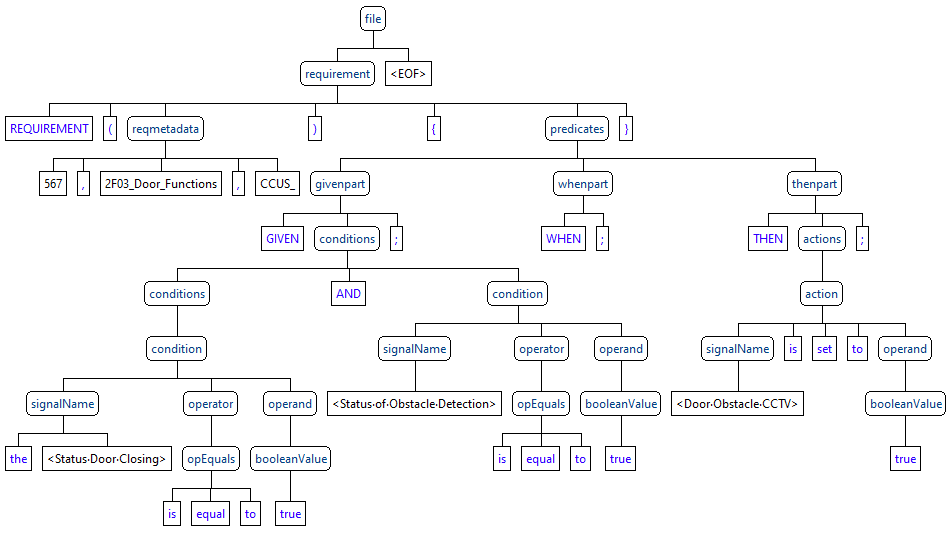
\includegraphics[scale=0.625]{images/parse_tree_req_example.PNG}
    \caption{Parse tree from the previous requirement example}
    \label{fig:req_parse_tree}
\end{figure}

The above requirement parsing has been benchmarked using the Eclipse IDE with ANTLR4 IDE 0.3.6 from the marketplace, resulting in the Figure \ref{fig:req_parse_tree}. Benchmark results are as follows:

\begin{table}[H]
\caption{ANTLR Grammar Profiler}
    \footnotesize
    \centering
    \begin{tabular}{c c c}
        \hline
        \textbf{\textit{Measurement}} & \textbf{\textit{Value}}\\ \hline
            &  \\
     \begin{tabular}[c]{@{}c@{}} \textbf{\textit{Input}} \textbf{\textit{Size}}\end{tabular}  & 198 chars, 6 lines  \\ \hline
        &   \\ 
       \textbf{\textit{ Number of Tokens}} & 34  \\ \hline
        &   \\
        \textbf{\textit{Parse Time (ms)}} & 2268 \\ \hline
            &   \\
        \textbf{\textit{Prediction Time (ms)}} & 0,711 = 31.36\%  \\ \hline
            &   \\
       \textbf{\textit{Lookahead Burden}} & 53/34 = 1.56  \\ \hline
        &  \\
       \textbf{\textit{DFA Cache miss rate}} &  \begin{tabular}[c]{@{}c@{}} 43/53 = 81.13\% \end{tabular}  \\ \hline
    \end{tabular}
    \label{tab:grammar_benchmark}
\end{table}

Before executing \textit{sesnando}, Debug mode can be enabled by setting the debug flag trough the command line. This will reduce the Log level and \textit{sesnando} will turn into a verbose execution by displaying the intermediate steps to the user. Next is a representation of the Parse tree from the Sesnando console output: \\

\lstset{language=XML}
\begin{lstlisting}
<?xml version="1.0" encoding="utf-8"?>
<AST>
  <RequirementSet>
    <Requirement>
      <Id>123456</Id>
      <TestCaseId>R151_2F03_DoorStat_TC_001</TestCaseId>
      <Namespace>MWT_</Namespace>
      <GivenConditions p4:type="ComparisonExpression">
        <ExpressionType>EXP_COMPARISON</ExpressionType>
        <ExpressionOperator>
          <ExpressionType>EXP_COMP_OPERATOR</ExpressionType>
          <OperatorType>OP_EQ</OperatorType>
        </ExpressionOperator>
        <LogicalSignal>
          <ExpressionType>EXP_SIGNAL</ExpressionType>
          <SignalName>CTC_OPDoorsFromMIO</SignalName>
          <SignalFormat>SIGNAL_ALIAS</SignalFormat>
        </LogicalSignal>
        <SignalValue>
          <ExpressionType>EXP_SIGNAL_VALUE</ExpressionType>
          <Type>SV_BOOL</Type>
          <Value>TRUE</Value>
        </SignalValue>
      </GivenConditions>
      <WhenConditions p4:type="EmptyLogicalExpression">
        <ExpressionType>EXP_EMPTY</ExpressionType>
      </WhenConditions>
      <ThenActions p4:type="ActionExpression">
        <ExpressionType>EXP_ACTION</ExpressionType>
        <LogicalSignal>
          <ExpressionType>EXP_SIGNAL</ExpressionType>
          <SignalName>CTC_STrcnSafeFromMIO</SignalName>
          <SignalFormat>SIGNAL_ALIAS</SignalFormat>
        </LogicalSignal>
        <SignalValue>
          <ExpressionType>EXP_SIGNAL_VALUE</ExpressionType>
          <Type>SV_BOOL</Type>
          <Value>TRUE</Value>
        </SignalValue>
        <Actor />
      </ThenActions>
    </Requirement>
  </RequirementSet>
</AST>
\end{lstlisting}
\label{code:xml_output}

The above XML tree has been automatically generated by extending the Object class in C\# and defining a new \textit{ToXMLString()} method which then uses the native XML Serializer.\\
The corresponding Object Tree will be stored on the the SESNANDO.Compiler.Common module, making it available to the remaining modules via a controller class.


\subsection{Test Generation}
%----------------------- Test Generation ----------------------------
\label{subsec:test_generation}

Test generator has two main roles: Translate each requirement signal into one or more software signals, and generate the combinatory explosion from the input signal values into test cases. Both procedures will be detailed on the next sub-sections.


\subsubsection{Signal Translation}
%----------------------- Signal Translation ----------------------------
\label{subsubsec:signal_translation}

As previously stated (Sec. \ref{subsec:requirement_processing}), a requirement is modeled and stored into an object tree. Next, the Test Generation module is called to access this tree and traverses it looking for Requirement Signals.

\begin{figure}[H]
    \centering
    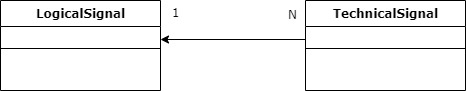
\includegraphics[scale=0.625]{images/class_diag_logical_technical_signal.jpg}
    \caption{LogicalSignal and TechnicalSignal class relationship}
    \label{fig:logical_technical_signal}
\end{figure}

Test generator accesses the signal manager trough an API endpoint, in the following format:\\
\textcolor{black}{https://<IP\_Address>:5001/api/signalByCore/<LogicalSignal>}\\
and will instantiate every \textit{Technical Signal} according to Signal Manager results. When a \textit{Logical signal} is not found, \textit{Sesnando} will report an error message to the user for the current requirement, as the signal must be added to the Database.


\subsubsection{Test case generation}
%----------------------- Test case generation ----------------------------
\label{subsubsec:test_cases}


For each requirement, \textit{Sesnando} extracts the \textit{Given} conditions as the test pre-conditions and \textit{When} conditions as the main input trigger according to the Railway project guidelines. Both predicates should evaluate to true in order to verify the expected results given by \textit{Then} predicate.\\

By default \textit{Sesnando} generates a set of test cases to positively test each input requirement. When a requirement is applied to a multiple set of components of the same type on the system, \textit{Sesnando} looks to test these components individually when a requirement instructs to do so, this is achieved through the use of quantifiers as it can be seen further. Next is an example of a requirement containing a quantifier.\\

\textit{
REQUIREMENT(567, 2F03\_Door\_Functions, CCUS) 
\{\\
	GIVEN <Status of Obstacle Detection> is equal to true \textbf{for at least one door of the train};\\
	WHEN;\\
	THEN <Door Obstacle alarm and CCTV> is set to true;\\
\}\\
}\\
\label{eq:requirement_quantifier}

For the pilot Railway project, a standard train unit contains (on maximum) twenty passenger doors. Using the example of the requirement above, \textit{Sesnando} understands that each door must be tested individually, given that each door reports its status whether an obstacle is detected and only one door signal needs to be true, for the \textit{Then} predicate to evaluate to true, so, testing all doors at once would be incorrect.\\

\begin{figure}[H]
    \centering
    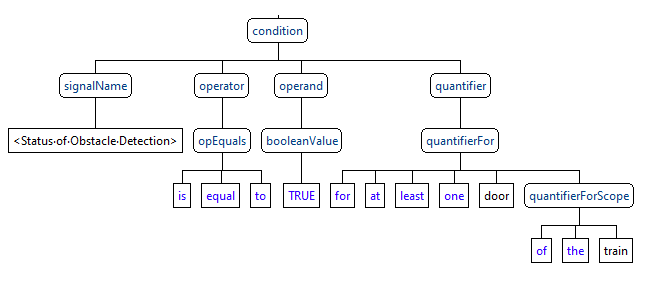
\includegraphics[scale=0.85]{images/quantifier_parse_tree.PNG}
    \caption{Requirement Quantifier Parse tree}
    \label{fig:quantifier_parse_tree}
\end{figure}

On the above diagram (Fig. \ref{fig:quantifier_parse_tree}), for the quantifier node, "for at least one" defined the type of the quantifier, \textit{Door} is the component/attribute of the signal and the train is the scope of the signal, meaning it is needs to be checked whether the present conditions evaluates to true for at least one door of the train. There are different types of quantifiers that can be used, such as "for all", "for exactly one" and "for the same" which will be discussed in detail on Sec. \ref{sec:method}.\\

\textit{Sesnando} supports three types of quantifiers.
\begin{itemize}
    \item "for one" - \textit{THEN} predicate evaluates to true if one and only one attribute/component within the quantifier evaluate to true.
        \begin{itemize}
            \item Example: Given <Status Train cab> is active \textbf{for one} cab of the train;\\
            When ...;\\
            Then ...;\\
        \end{itemize}
    \item "for at least" - \textit{THEN} predicate evaluates to true if at least one attribute/component within the quantifier evaluate to true.
        \begin{itemize}
            \item Example: Given <Status door> is open \textbf{for at least} one door of the train;\\
            When ...;\\
            Then ...;\\
        \end{itemize}
    \item "for all" - \textit{THEN} predicate evaluates to true if all attributes/components within
    the quantifier evaluate to true.
        \begin{itemize}
            \item Example: Given <Status Emergency brake> is applied \textbf{for all} brakes of the train;\\
            When ...;\\
            Then ...;\\
        \end{itemize}
\end{itemize}

A requirement suports multiple conditions and each condition supports only one quantifier.
The generation of test cases for a requirement containing a single quantifier, is given by the following equation.

\begin{equation}
    \text{input}[i] = true \quad \forall i \in \{0, 1, \dots , n-1\}
\end{equation}
\label{eq1}

A deeper representation of multiple signals and quantifiers combined, is given by \textit{Hadamard} Product matrices, resulting in the following equations.


\begin{equation}
    \text{out} = \text{inp} \circ \text{inp}
\end{equation}
\label{eq2}

Where the output result, hence, the expected results is given by \textit{out}.

\begin{equation}
\text{out} = ReqSignalN \circ ReqSignalK = (a_{ij}\cdot b_i) = 
\begin{pmatrix} 
a_{11} \cdot b_{1} & \cdots & a_{1n} \cdot b_{1} \\
\vdots & \ddots & \vdots \\ 
a_{m1} \cdot b_{m} & \cdots & a_{mn} \cdot b_{m} 
\end{pmatrix}
\end{equation}

So that, for instance, a scalar Requirement condition and a Quantified Requirement condition, both evaluating to true when using an \textit{AND} operator would result in the following expected result.

\begin{equation}
\begin{pmatrix}
1 & 0 & 0\\
0 & 1 & 0\\
0 & 0 & 1
\end{pmatrix} = 
\begin{pmatrix}
1\\
1\\
1 
\end{pmatrix} 
\begin{pmatrix}
1 & 0 & 0\\
0 & 1 & 0\\
0 & 0 & 1
\end{pmatrix} 
\end{equation}\\

According to the requirement guidelines defined in the Railway project that is being used as a pilot to validate this tool, the writing of OR conditions is highly discouraged, hence, \textit{Sesnando} does not allow for requirements containing OR conditions to be included in the input file. For cases where a requirement contains an OR operator, those requirements shall be re-written into multiple requirements. \textcolor{red}{a menos que até lá se inclua uma feature para executar a AST e procurar re-avaliar os expected results re-exercitando os inputs na AST e predir uma nova avaliação da tree (isto fará parte da execução natural do Sesnando e não opcional usando robustness testing)}.\\


\subsection{Signal Manager}
%----------------------- Signal Manager ----------------------------
\label{subsec:signal_manager}

Ideally, \textit{Signal Manager} should run on a remote server where the testing information is centralized. The main benefits of this approach is that every tester, developer or project stake-holder can contribute to develop a solid knowledge base to sustain the test generation from \textit{Sesnando Compiler} instance.\\

\textit{Signal Manager} can be accessed trough a Web Interface running on port 5001. From there, the user is able to edit Technical signals (Software signals) which can be mapped to the corresponding Logical Signals (Requirement Signals) as well as add relevant data like attributes and states. See (Fig. \ref{fig:signal_manager_pibs})

\begin{figure}[H]
    \centering
    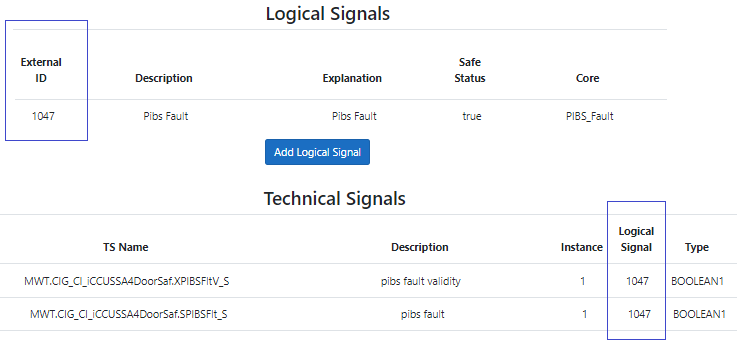
\includegraphics[width=\textwidth]{images/signal_manager_signals_pibs.PNG}
    \caption{Signal Manager PIBS Signal Mapping example}
    \label{fig:signal_manager_pibs}
\end{figure}

The Figure \ref{fig:signal_manager_pibs} is an excerpt from the \textit{Signal Manager} interface. It can be seen that a set of technical signals are mapped to a Logical Signal trough an Id value. A Technical signal might accept several attributes, e.g., a door \textit{Side} or Car location within the train or a state, e.g., Open, Released, Closed, that might be represented through an integer number, this is defined from the original requirement, e.g., "Given <Door status> is equal to Released".


\subsection{Test Designer}
%----------------------- Test Designer ----------------------------
\label{subsec:test_designer}

The main goal of \textit{Test Designer} is to display the generated test specification to the user. The user is able to modify it as intended and from there, generate a test script. This interface is presented on the next image (Fig. \ref{fig:test_designer_interface}).

\begin{figure}[H]
    \centering
    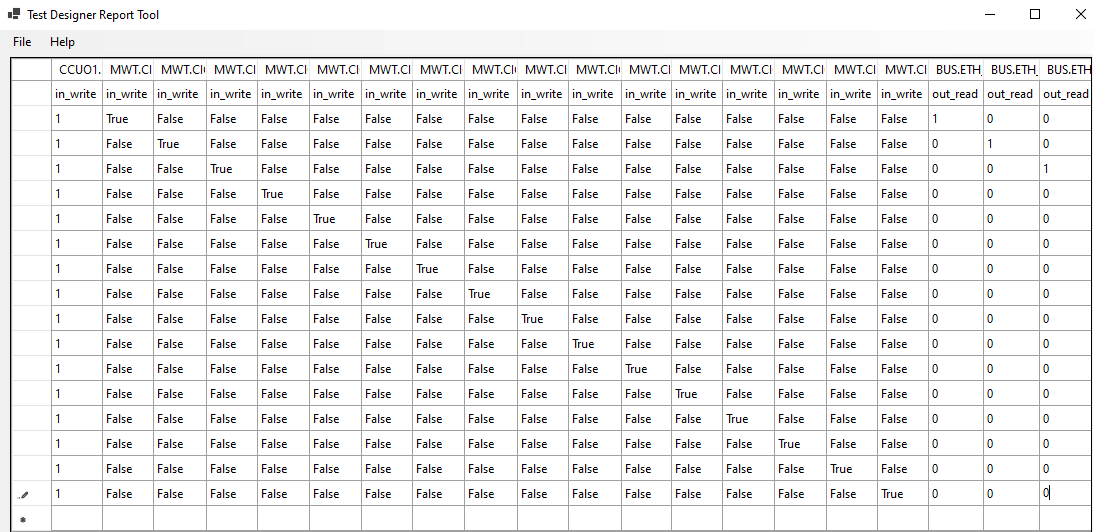
\includegraphics[width=\textwidth]{images/test_designer.PNG}
    \caption{Test Designer Interface}
    \label{fig:test_designer_interface}
\end{figure}

The above image (Fig. \ref{fig:test_designer_interface}) is the result of a scalar requirement signal evaluating to int value "1" combined with an \textit{AND} operator to a quantifier requirement signal. Tests are executed from top to bottom.
The first row of the table corresponds to the software technical signal, the second row defines the direction of the signal as:

\begin{itemize}
    \item in\_write - The value to be \textit{forced} on the corresponding technical signal.
    \item out\_write - The expected results according the test inputs from the left input columns.
\end{itemize}


\subsubsection{Generated Artifacts and test execution}
%----------------------- Generated Artifacts ----------------------------
\label{subsubsec:generated_artifacts}

After visualising and reviewing the test specification on the test designer, the tester will be able to export it into a test script compatible with the test execution tool. This feature can be located by navigating to "File -> Export to test script". At this moment \textit{Sesnando} only supports one script type but it is intended that the user interface could be extended to support multiple script types as needed.\\
With this, it is intended to demonstrate a complete end-to-end lifecycle, from requirements to test execution. Next, is a tool that allows the observation of the internal states of a simulated train in operation (Fig. \ref{fig:test_environment})

\begin{figure}[H]
    \centering
    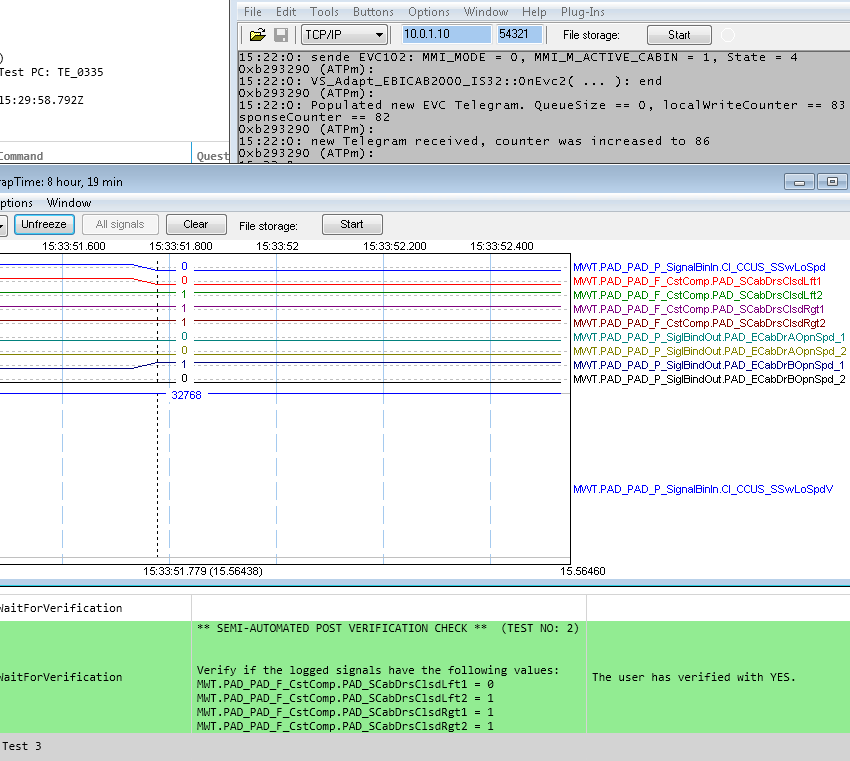
\includegraphics[width=\textwidth]{images/test_environment.png}
    \caption{Test Environment}
    \label{fig:test_environment}
\end{figure}

The validation facility loads the script generated from \textit{Sesnando} and is able to connect to the test environment through a TCP Socket. On a simple operation, the signal values start to be set on the software to produce the desire outcomes. The real-time value of every software signal through the test time-span can be observed on the multi-chart present on the software tool (Fig. \ref{fig:test_environment}). This also demonstrates that \textit{Sesnando} is able to generate test scripts from the input requirements that are compatible with the presented test environment.




